\section{Initially Random, Greedy Deployment}
\label{sec:initially_random_greedy}

Combining the random and greedy deployment schemes allows us to inject uncertainty as to which reactor will be deployed at any given time while ensuring that the demand is met efficiently. This scheme does not give us more insight than the random or greedy deployment; it merely allows us to leverage the strengths of both.

This deployment scheme randomly deploys reactors until a reactor bigger than the remaining capacity is proposed for each year, then it fills the remaining capacity with a greedy algorithm. Figure \ref{fig:init_random_greedy_diagram} outlines, which shows the two loops (first random, then greedy) in the logic from the top down.

\begin{figure}[H]
  \centering
  \begin{tikzpicture}[node distance = 2.5cm, auto]
    % Place random nodes
    \node [block] (init) {\textbf{Initialize demand.}};
    \node [block, below of=init, node distance=2.5cm] (evaluate) {\textbf{Randomly deploy one reactor.}};
    \node [block, right of=evaluate, node distance=3.5cm] (update) {\textbf{Does this reactor exceed demand?}};
    % Place greedy nodes
    \node [block, below of=update] (checkg) {\textbf{Is there demand?}};
    \node [block, below of=checkg, node distance=2.5cm] (evaluateg) {\textbf{Deploy the largest capacity reactor below demand.}};
    \node [block, below of=evaluateg, node distance=2.5cm] (updateg) {\textbf{Update demand.}};
    \node [block, left of=checkg, node distance=4cm] (stopg) {\textbf{Next time step.}};
    % Draw edges
    \path [line, line width=0.6mm] (init) -- (evaluate);
    \path [line, line width=0.6mm] (evaluate) -- (update);
    \draw[->, line width=0.6mm] (update) -- node[left]{\textbf{Yes}}(checkg);
    \draw[->, line width=0.6mm] (update) edge[bend right=65] node[above]{\textbf{No}} (evaluate);
    % Draw greedy edges
    \path [line, line width=0.6mm] (checkg) -- node {\textbf{Yes}} (evaluateg);
    \path [line, line width=0.6mm] (evaluateg) -- (updateg);
    \path [line, line width=0.6mm] (checkg) -- node {\textbf{No}}(stopg);
    \draw[->, line width=0.6mm] (updateg) edge[bend right=65] node[right]{} (checkg);
  \end{tikzpicture}
  \caption{The initially random, greedy deployment diagram demonstrates how the random and greedy deployment schemes complement each other for a single time step.}
  \label{fig:init_random_greedy_diagram}
\end{figure}

% \begin{figure}[H]
%     \centering
%     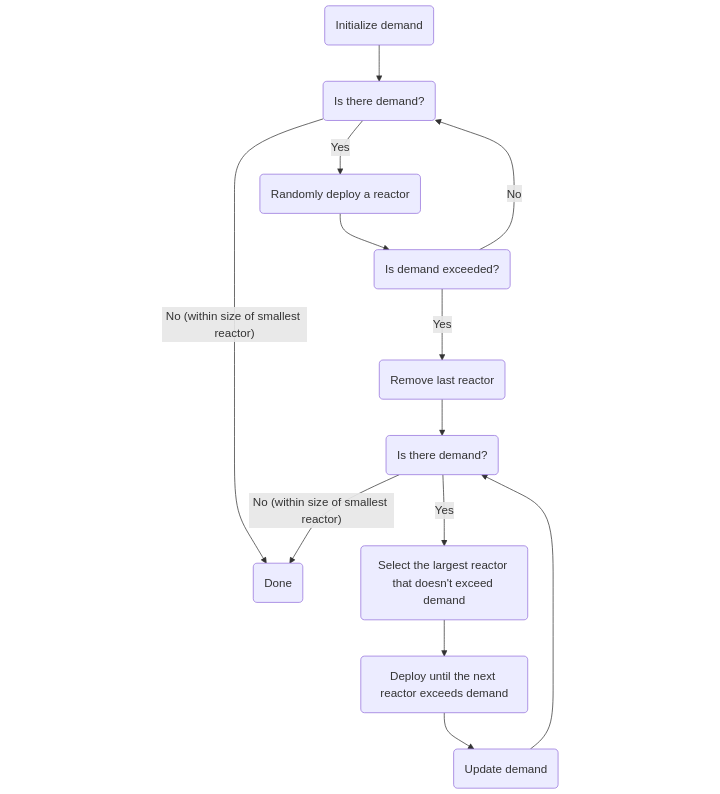
\includegraphics[scale=0.55]{images/schemes/random_greedy_diagram.png}
%     \caption{Initially random, greedy deployment diagram.}
%     \label{fig:init_random_greedy_diagram}
% \end{figure}

Section \ref{sec:random_deployment} highlights how this thesis did not implement the initially random, greedy deployment scheme to capture additional realism in the deployment problem. This scheme combines random and greedy deployment schemes and inherits their realistic and unrealistic elements. The random deployment scheme captures some of the complexity of the deployment problem but does not guarantee the capture of the nuance of future user needs. The greedy deployment scheme captures the efficiency of the deployment problem but does not capture the complexity of the deployment problem. This scheme is a compromise between the two and does not capture the nuance of the deployment problem.

The seed, which was set to 20240527121205 for every run for this scheme, for
the random number generator is set by the date and time of the simulation,
which allows for the reproducibility of the results. The degree to which this
scheme captures features of the random or greedy deployment schemes varies with
the number of reactors deployed in the random phase. Instead of randomly
deploying until the demand is met, this implementation randomly deploys until
the selected reactor exceeds the demand. This means that when the reactors are
different sizes, there is a chance that the random phase will deploy a reactor
larger than the demand, and the greedy phase will make up more of
the deployment.


\subsection{Number of Reactors}
\label{sec:rand_greed_reactors}

As with the random deployment scheme, Figures
\ref{fig:rand_greed_mf_reactors} and \ref{fig:rand_greed_of_reactors} show that the share of reactors by design is much closer than the greedy deployment scheme. The reactors in the \textit{no growth} scenarios (shown in Figures \ref{fig:rand_greed_mf_ng} and \ref{fig:rand_greed_of_ng}) are deployed close to 2050, whereas the advanced reactors in the \textit{double by 2050} scenarios (shown in Figures \ref{fig:rand_greed_mf_d2} and \ref{fig:rand_greed_of_d2}) are deployed close to 2030.

% Show total number of reactors multi-fuel
\begin{figure}[H]
    \subfloat[No Growth. \label{fig:rand_greed_mf_ng_reactors}]{%
      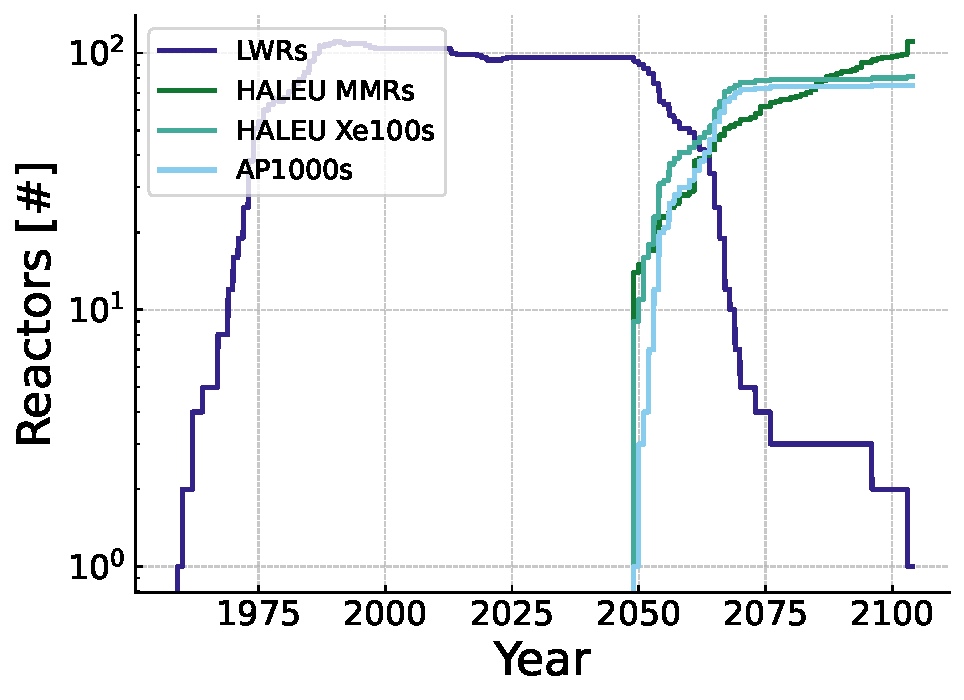
\includegraphics[width=0.495\textwidth]{images/results/reactors/multi_drgng_reactors.pdf}
   }
    \hfill
    \subfloat[Double. \label{fig:rand_greed_mf_d2_reactors}]{%
      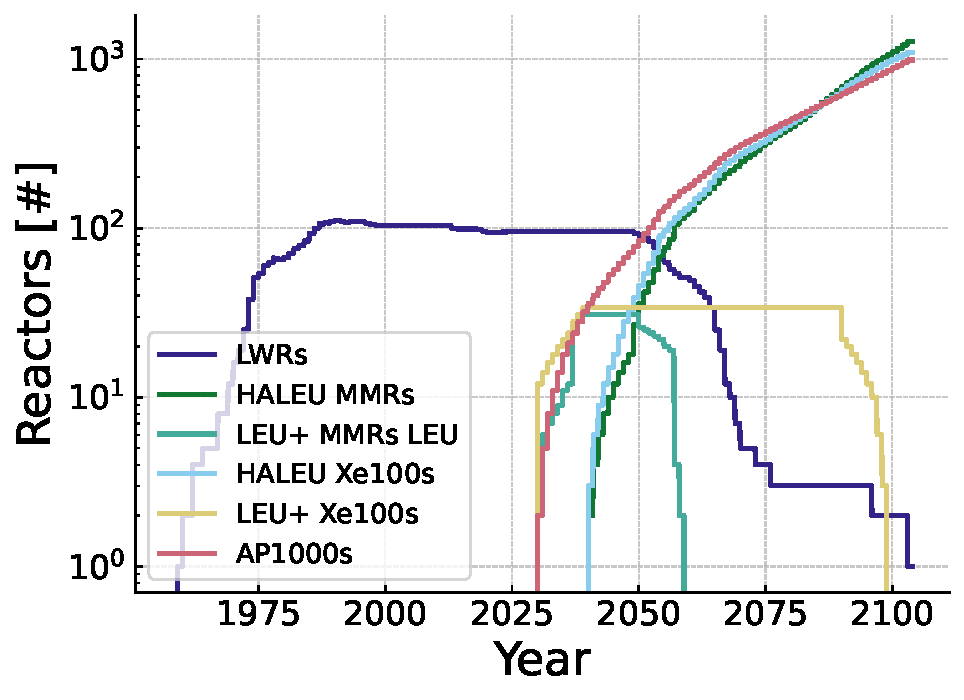
\includegraphics[width=0.495\textwidth]{images/results/reactors/multi_drg2_reactors.pdf}
   }
    \caption{Multiple fuels initially random, then greedy reactor deployment.}
    \label{fig:rand_greed_mf_reactors}
  \end{figure}

% talk about the rate of deployment

% talk about the context of expanding energy needs

% talk about the workers

\begin{figure}[H]
    \subfloat[No Growth. \label{fig:rand_greed_of_ng_reactors}]{%
      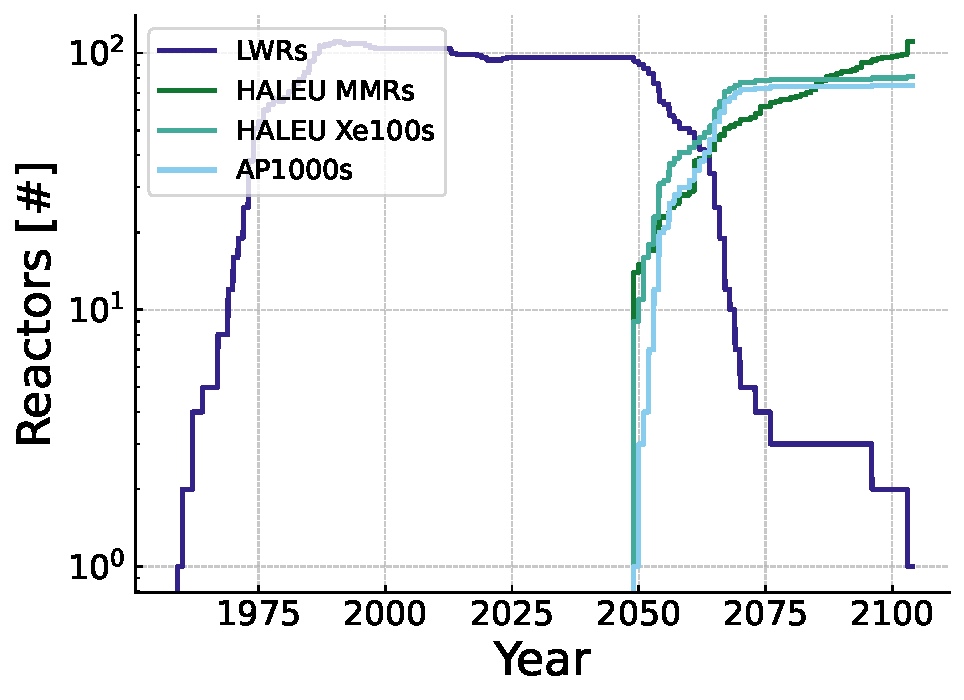
\includegraphics[width=0.495\textwidth]{images/results/reactors/one_drgng_reactors.pdf}
   }
    \hfill
    \subfloat[Double. \label{fig:rand_greed_of_d2_reactors}]{%
      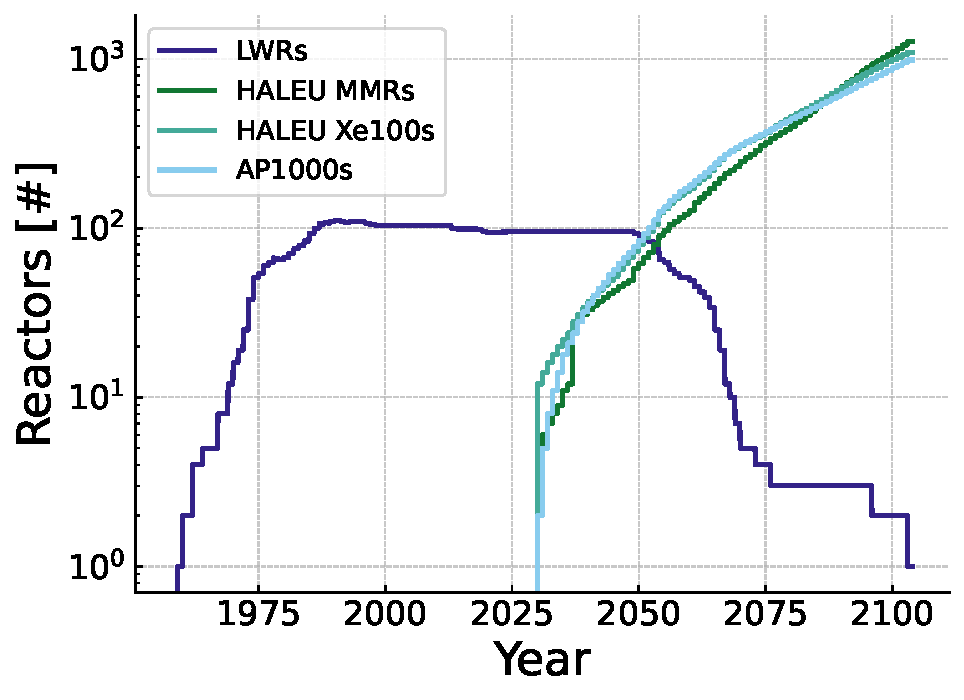
\includegraphics[width=0.495\textwidth]{images/results/reactors/one_drg2_reactors.pdf}
   }
    \caption{Single-fuel initially random, then greedy reactor deployment.}
    \label{fig:rand_greed_of_reactors}
\end{figure}

Table \ref{tab:rand_greed_reac_avg} shows the average total operating reactors by design for the \textit{no growth} and \textit{double by 2050} scenarios for the multi and single-fuel enrichment deployments. The \gls{haleu} fueled \gls{mmr} and \gls{xe} deployment is unchanged in the single and multi-fuel enrichment deployments for the \textit{no growth} scenarios. The number of AP1000 reactors increases 660\% from the \textit{no growth} to the \textit{double by 2050} scenario in the multi-fuel enrichment deployment. The number of \gls{haleu} fueled \gls{xe} reactors increases 626\%, while the number of \gls{haleu} fueled \gls{mmr} reactors increases 649\%.

\begin{table}[H]
    \centering
    \caption{Average initially random, then greedy total operating reactors by design.}
    \label{tab:rand_greed_reac_avg}
    \begin{tabular}{l c c c c}
       \toprule
       Scenario & \shortstack{No Growth,\\ Single} & \shortstack{No Growth,\\ Multiple} & \shortstack{Double,\\ Single} & \shortstack{Double,\\ Multiple}  \\
       \midrule
       \gls{haleu} fueled MMRs      & \textcolor{white}{0}44.547  & \textcolor{white}{0}44.547  & 333.613 & 325.347 \\
       \gls{leup} fueled MMRs       & --      & --      & --      & \textcolor{white}{00}8.267   \\
       \gls{haleu} fueled \gls{xe}s & \textcolor{white}{0}47.52   & \textcolor{white}{0}47.52   & 344.88  & 317.68  \\
       \gls{leup} fueled \gls{xe}s  & --      & --      & --      & \textcolor{white}{0}27.2    \\
       \gls{leu} fueled AP1000      & \textcolor{white}{0}42.72   & \textcolor{white}{0}42.72   & 324.68  & 324.68  \\
       \bottomrule
    \end{tabular}
\end{table}

\subsection{SWU Results}
\label{sec:rand_greed_swu}

Figure \ref{fig:swu_yearly_rand_greed} shows the yearly \gls{swu} demand periodically spike as reactors begin operation in the depicted \textit{no growth} scenario around 2050. The \gls{swu} demand for the AP1000 \gls{leu} rises above the other two reactors while the demand from \glspl{xe} overlaps heavily with the demand from \glspl{mmr}. This trend is exacerbated in the \textit{double by 2050} scenarios shown in Figures \ref{fig:rand_greed_mf_d2_swu} and \ref{fig:rand_greed_of_d2_swu} where the \gls{swu} for AP1000 \gls{leu} fuel rises quickly and eventually exceeds the total \gls{swu} for the existing fleet.
% talk about the SWU capacity

% show the total SWU capacity
\begin{figure}[H]
    \centering
    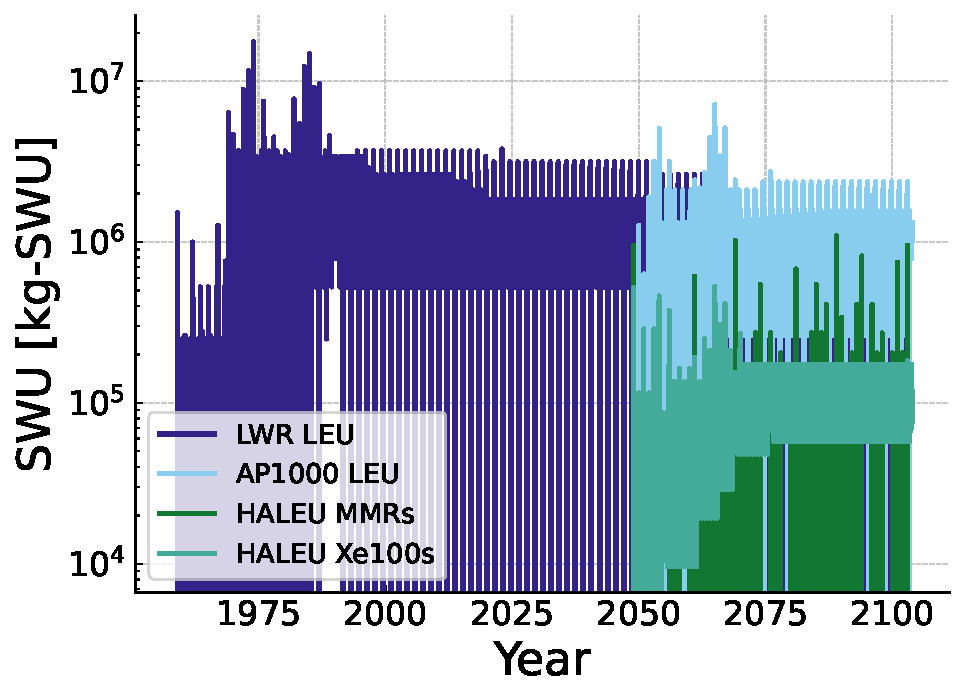
\includegraphics[scale=0.7]{images/results/swu/multi_drgng_swu_by_fuel.pdf}
    \caption{Initially random, then greedy yearly SWU demand.}
    \label{fig:swu_yearly_rand_greed}
\end{figure}

As the features of the yearly data are regular, dictated by the cycles of the reactors, and overlapping, Figures \ref{fig:rand_greed_mf_swu} and \ref{fig:rand_greed_of_swu} visualize the total cumulative \gls{swu} demand.


\begin{figure}[H]
  \subfloat[No Growth. \label{fig:rand_greed_mf_ng_swu}]{%
    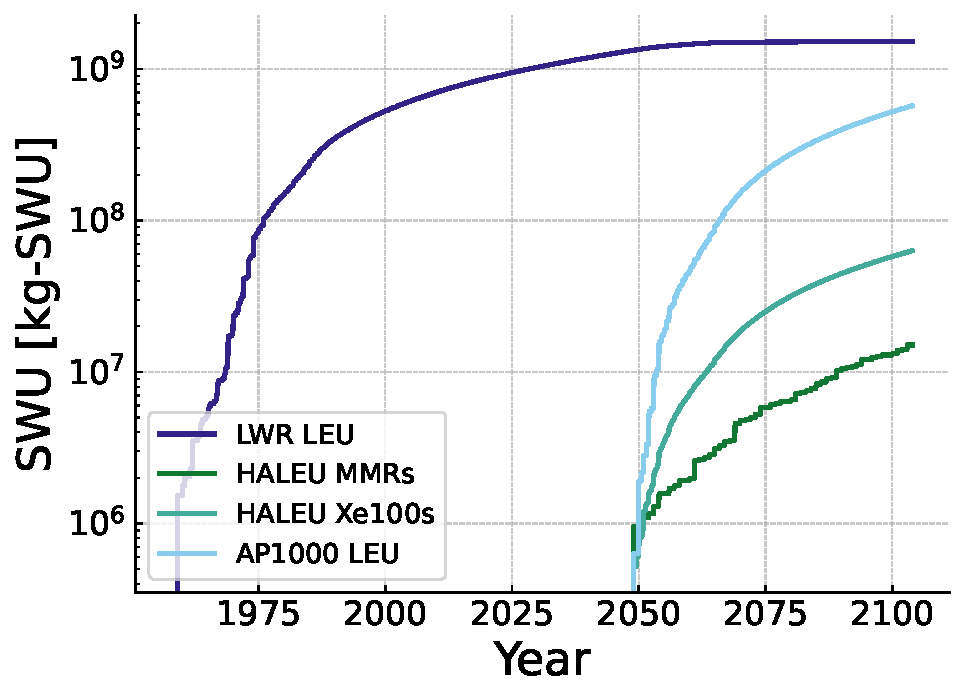
\includegraphics[width=0.495\textwidth]{images/results/swu/multi_drgng_swu_cumulative_by_fuel.pdf}
 }
  \hfill
  \subfloat[Double. \label{fig:rand_greed_mf_d2_swu}]{%
    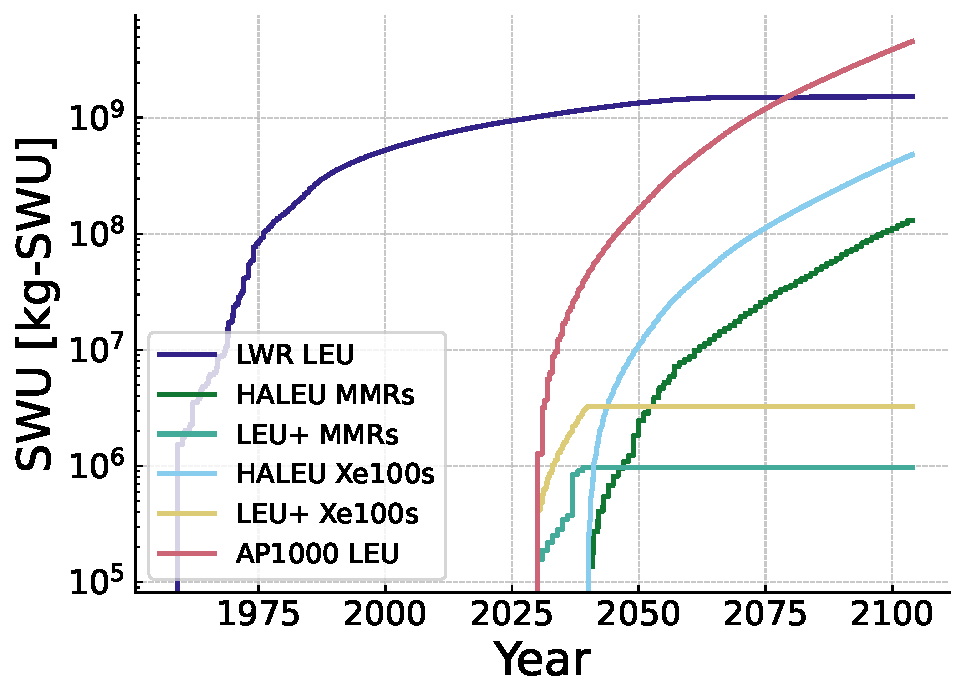
\includegraphics[width=0.495\textwidth]{images/results/swu/multi_drg2_swu_cumulative_by_fuel.pdf}
 }
  \caption{Initially random, then greedy multi-fuel SWU.}
  \label{fig:rand_greed_mf_swu}
\end{figure}



\begin{figure}[H]
    \subfloat[No Growth. \label{fig:rand_greed_of_ng_swu}]{%
      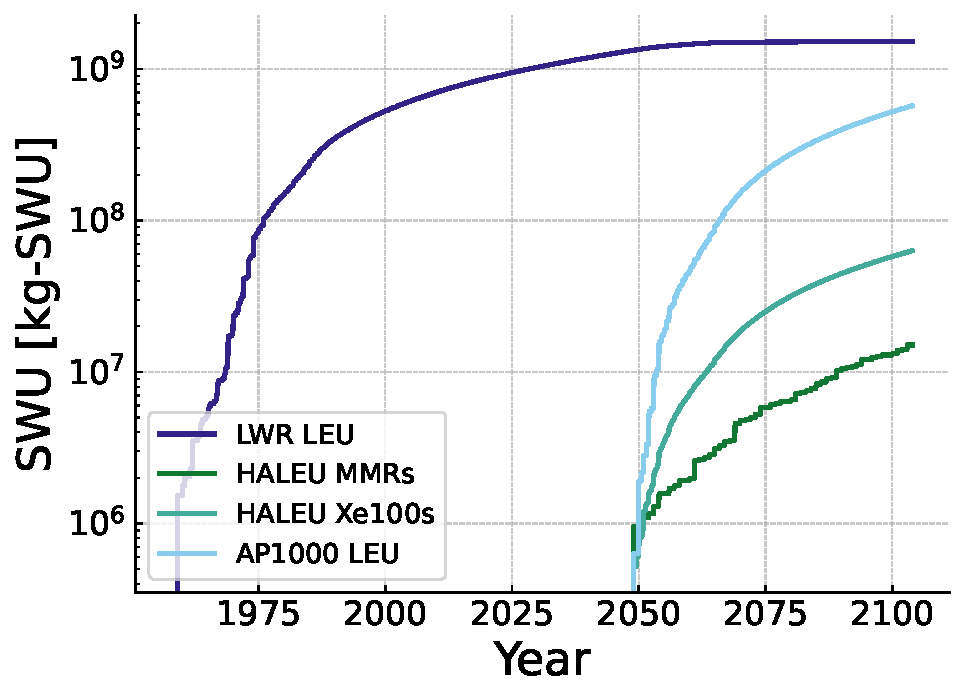
\includegraphics[width=0.495\textwidth]{images/results/swu/one_drgng_swu_cumulative_by_fuel.pdf}
   }
    \hfill
    \subfloat[Double. \label{fig:rand_greed_of_d2_swu}]{%
      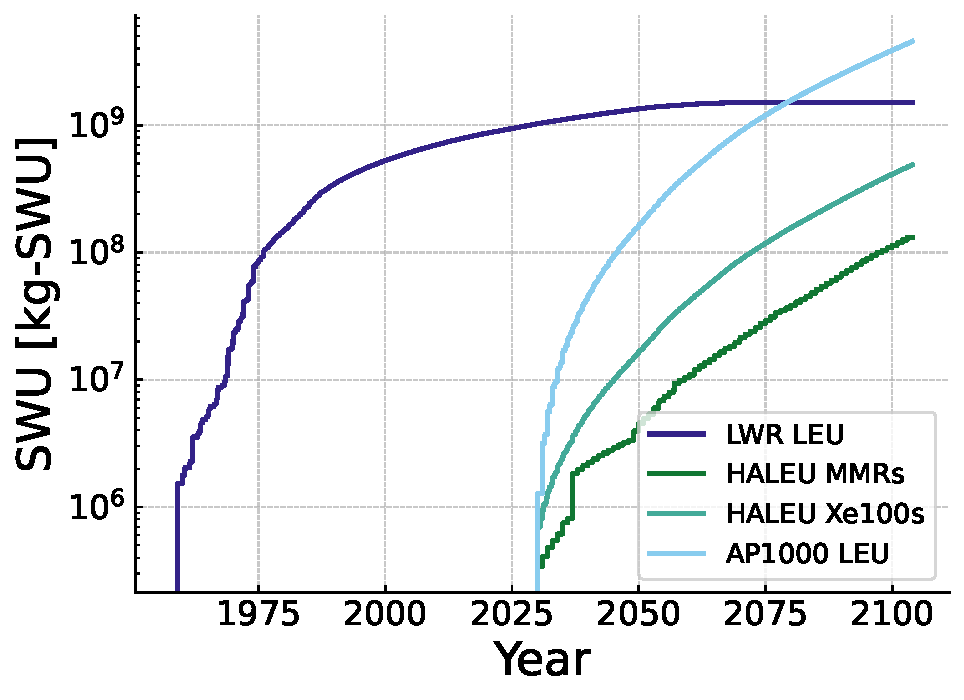
\includegraphics[width=0.495\textwidth]{images/results/swu/one_drg2_swu_cumulative_by_fuel.pdf}
   }
    \caption{Initially random, then greedy single-fuel SWU.}
    \label{fig:rand_greed_of_swu}
\end{figure}

% talk about international trade

Table \ref{tab:rand_greed_swu_avg} shows the average yearly \gls{swu} for the \textit{no growth} and \textit{double by 2050} scenarios for the multi and single-fuel enrichment deployments. The \gls{swu} demand for the \gls{mmr} and \gls{xe} reactors is the same in the single and multi-fuel enrichment deployments for the \textit{no growth} scenarios, which is consistent with the reactor deployment trends in the Section \ref{sec:rand_greed_reactors}. Across scenarios, the demand for \gls{swu} for AP1000 \gls{leu} fuel increases 696\% from the \textit{no growth} to the \textit{double by 2050} scenario in the single-fuel enrichment deployment. The demand for \gls{swu} for \gls{haleu} fuel in the \gls{mmr} and \gls{xe} reactors increases 775\% and 672\% respectively from the \textit{no growth} to the \textit{double by 2050} scenario in the multi-fuel enrichment deployment.

\begin{table}[H]
    \centering
    \caption{Average initially random, then greedy yearly SWU by design in k\gls{swu}.}
    \label{tab:rand_greed_swu_avg}
    \begin{tabular}{l c c c c}
       \toprule
       Scenario & \shortstack{No Growth,\\ Single} & \shortstack{No Growth,\\ Multiple} & \shortstack{Double,\\ Single} & \shortstack{Double,\\ Multiple}  \\
       \midrule
       \gls{mmr} \gls{haleu}   & \textcolor{white}{00}16.738  & \textcolor{white}{00}16.738  & \textcolor{white}{0}146.477  & \textcolor{white}{0}144.129  \\
       \gls{mmr} \gls{leup}    & --      & --      & --       & \textcolor{white}{000}1.079    \\
       \gls{xe} \gls{haleu}    & \textcolor{white}{00}70.066  & \textcolor{white}{00}70.066  & \textcolor{white}{0}540.613  & \textcolor{white}{0}534.559  \\
       \gls{xe} \gls{leup}     & --      & --      & --       & \textcolor{white}{000}3.624    \\
       AP1000 \gls{leu}        & \textcolor{white}{0}634.553 & \textcolor{white}{0}634.553 & 5050.323 & 5050.323 \\
       \bottomrule
    \end{tabular}
\end{table}



\subsection{Fresh Fuel Results}
\label{sec:rand_greed_fresh}

% talk about the types of fuel
Figures \ref{fig:rand_greed_mf_fresh} and \ref{fig:rand_greed_of_fresh} show the fresh fuel demand for the reactors in the \textit{no growth} and \textit{double by 2050} scenarios. The fresh fuel curves in each scenario follow the same pattern as the reactor deployment curves from Figures \ref{fig:rand_greed_mf_reactors} and \ref{fig:rand_greed_of_reactors}, as \cyclus supplies fuel to each of the reactors as it they deploy.


% show total fresh fuel
\begin{figure}[H]
    \subfloat[No Growth. \label{fig:rand_greed_mf_ng_fresh}]{%
      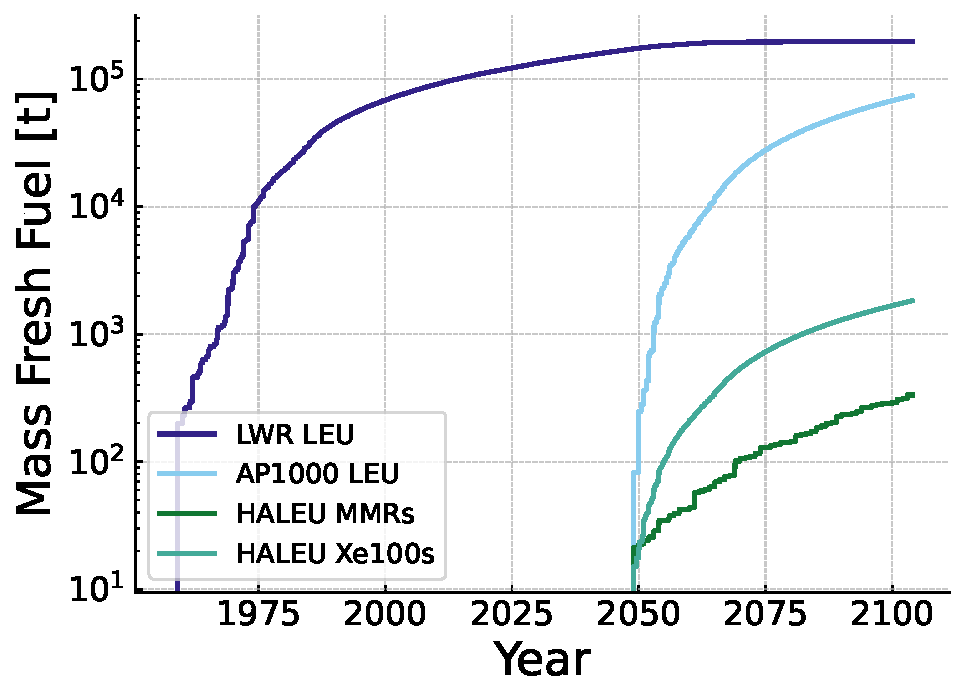
\includegraphics[width=0.495\textwidth]{images/results/fresh/multi_drgng_fresh_fuel_cumulative_by_fuel.pdf}
   }
    \hfill
    \subfloat[Double. \label{fig:rand_greed_mf_d2_fresh}]{%
      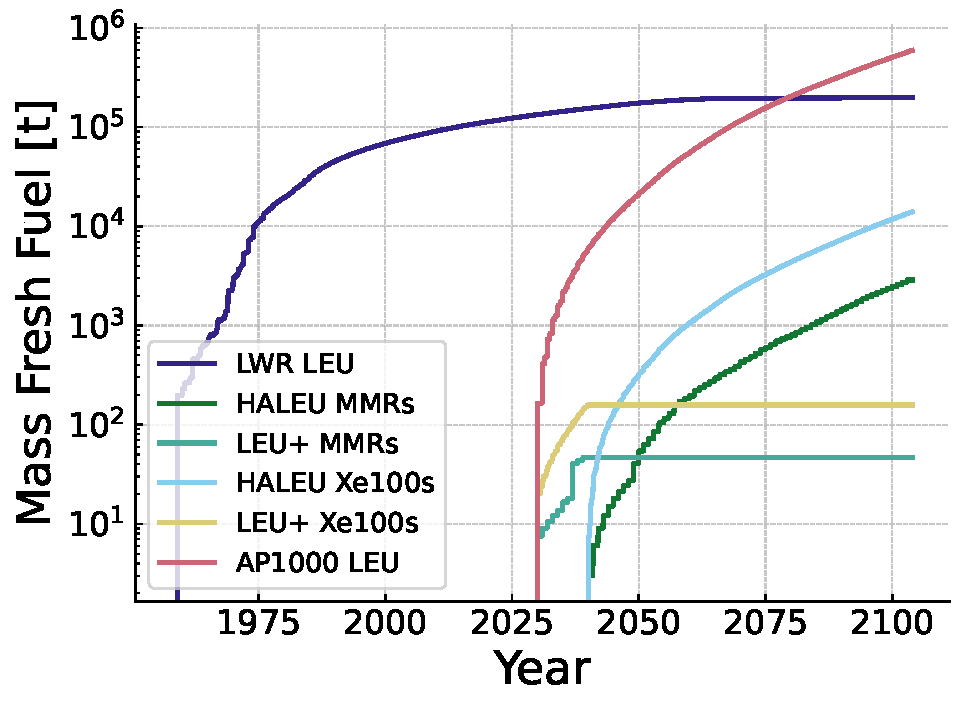
\includegraphics[width=0.495\textwidth]{images/results/fresh/multi_drg2_fresh_fuel_cumulative_by_fuel.pdf}
   }
    \caption{Initially random, then greedy multi fresh fuel demanded.}
    \label{fig:rand_greed_mf_fresh}
  \end{figure}

% talk about transportation of fuel


\begin{figure}[H]
    \subfloat[No Growth. \label{fig:rand_greed_of_ng_fresh}]{%
      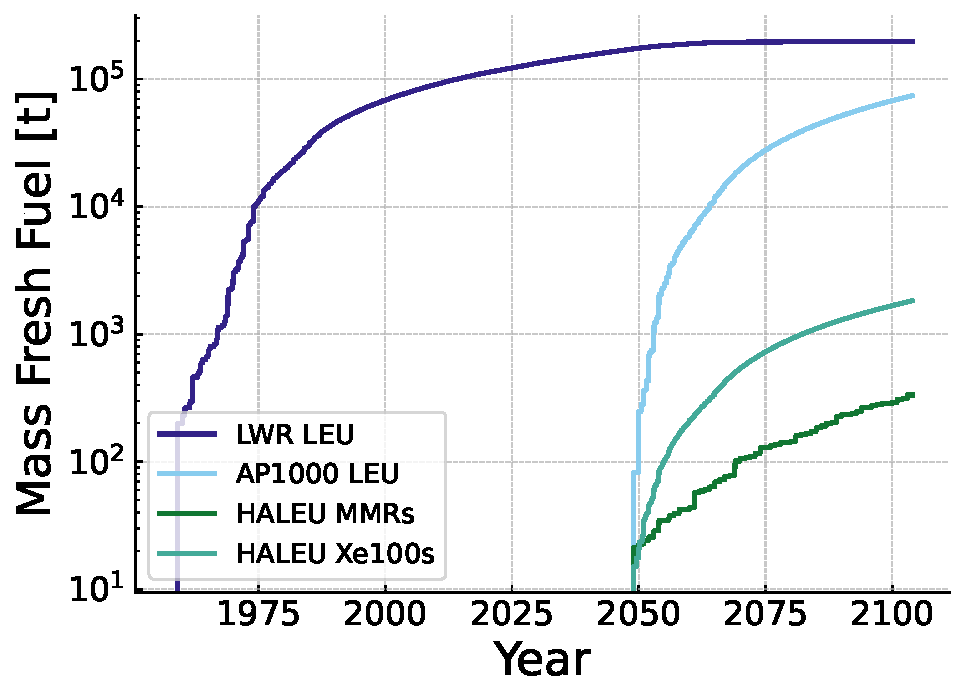
\includegraphics[width=0.495\textwidth]{images/results/fresh/one_drgng_fresh_fuel_cumulative_by_fuel.pdf}
   }
    \hfill
    \subfloat[Double. \label{fig:rand_greed_of_d2_fresh}]{%
      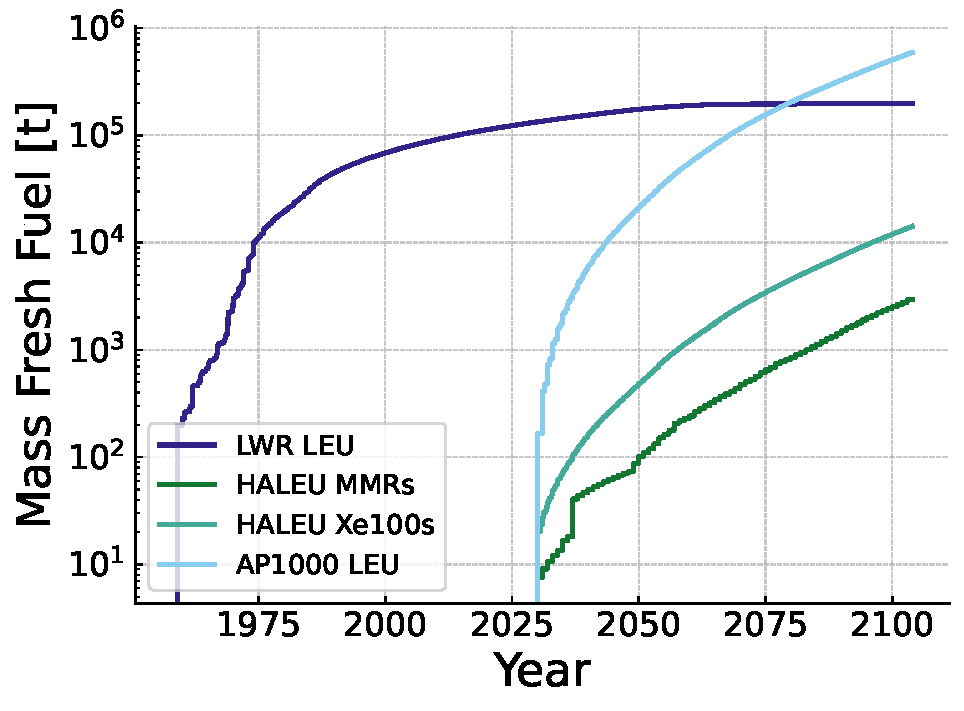
\includegraphics[width=0.495\textwidth]{images/results/fresh/one_drg2_fresh_fuel_cumulative_by_fuel.pdf}
   }
    \caption{Initially random, then greedy single fresh fuel demanded.}
    \label{fig:rand_greed_of_fresh}
  \end{figure}

Table \ref{tab:rand_greed_fresh_avg} shows the average yearly fresh fuel by design in tonnes for the \textit{no growth} and \textit{double by 2050} scenarios for the multi and single-fuel enrichment deployments. The fresh fuel demand for the reactors is the same in the single and multi-fuel enrichment deployments for the \textit{no growth} scenarios, which is consistent with the reactor deployment trends in the Section \ref{sec:rand_greed_reactors}. Across scenarios, the demand for fresh fuel for AP1000 \gls{leu} fuel increases 696\% from the \textit{no growth} to the \textit{double by 2050} scenario in the single-fuel enrichment deployment. The demand for fresh fuel for \gls{haleu} fuel in the \gls{mmr} and \gls{xe} reactors increases 775\% and 671\% respectively from the \textit{no growth} to the \textit{double by 2050} scenario in the multi-fuel enrichment deployment.

\begin{table}[H]
    \centering
    \caption{Average initially random, then greedy yearly fresh fuel by design in tonnes.}
    \label{tab:rand_greed_fresh_avg}
    \begin{tabular}{l c c c c}
       \toprule
       Scenario & \shortstack{No Growth,\\ Single} & \shortstack{No Growth,\\ Multiple} & \shortstack{Double,\\ Single} & \shortstack{Double,\\ Multiple}  \\
       \midrule
       \gls{mmr} \gls{haleu}   & \textcolor{white}{00}0.371    & \textcolor{white}{00}0.371   & \textcolor{white}{00}3.247    & \textcolor{white}{00}3.194    \\
       \gls{mmr} \gls{leup}    & --       & --      & --       & \textcolor{white}{00}0.052    \\
       \gls{xe} \gls{haleu}    & \textcolor{white}{00}2.033    & \textcolor{white}{00}2.033   & \textcolor{white}{0}15.683   & \textcolor{white}{0}15.507   \\
       \gls{xe} \gls{leup}     & --       & --      & --       & \textcolor{white}{00}0.176    \\
       AP1000 \gls{leu}        & \textcolor{white}{0}82.512   & \textcolor{white}{0}82.512  & 656.698  & 656.698  \\
       \bottomrule
    \end{tabular}
\end{table}


\subsection{Used Fuel Results}
\label{sec:rand_greed_used}

Figures \ref{fig:rand_greed_mf_used} and \ref{fig:rand_greed_of_used} depict the used fuel accumulation for the reactors in the \textit{no growth} and \textit{double by 2050} scenarios. The used fuel curves in each scenario follow the reactor deployment curves with a lag corresponding to the cycle length of the reactor from Figures \ref{fig:rand_greed_mf_reactors} and \ref{fig:rand_greed_of_reactors}, as \cyclus removes fuel from each reactor.


% show total used fuel
\begin{figure}[H]
    \subfloat[No Growth. \label{fig:rand_greed_mf_ng_used}]{%
      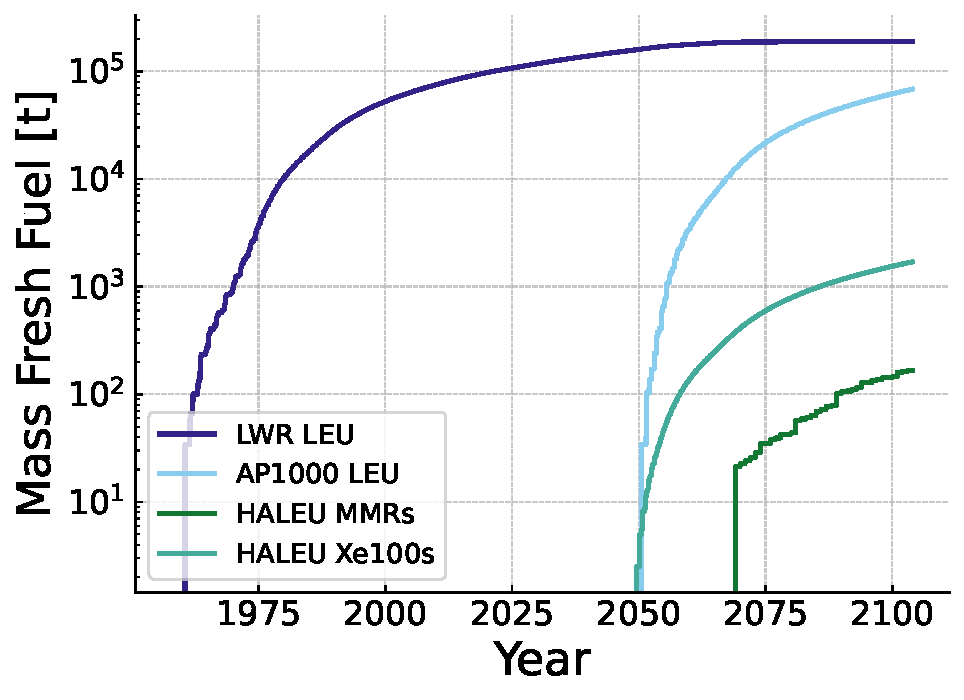
\includegraphics[width=0.495\textwidth]{images/results/used/multi_drgng_used_fuel_cumulative_by_fuel.pdf}
   }
    \hfill
    \subfloat[Double. \label{fig:rand_greed_mf_d2_used}]{%
      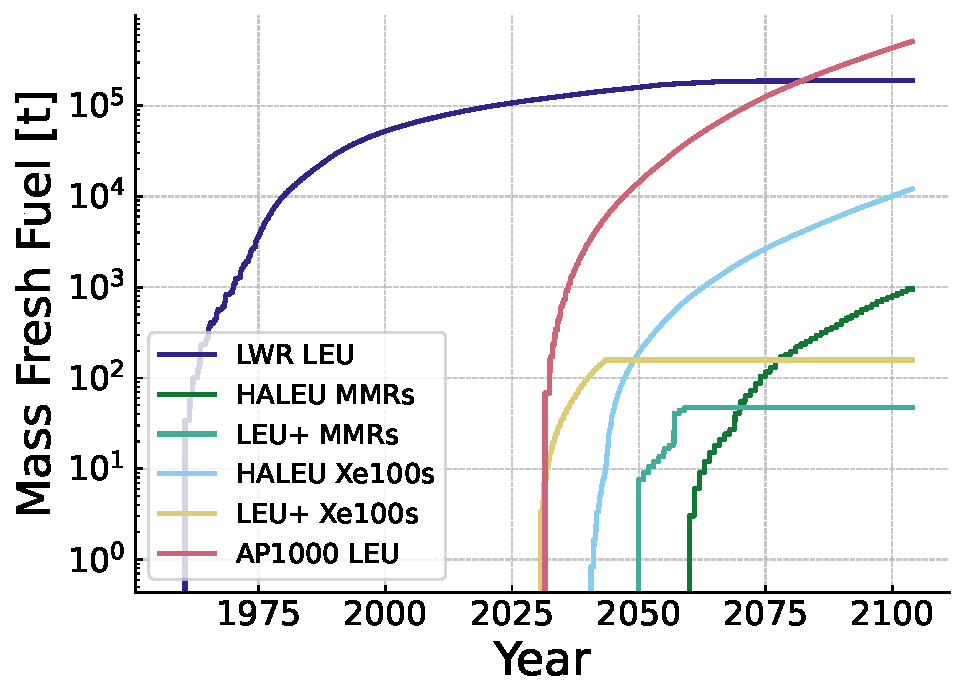
\includegraphics[width=0.495\textwidth]{images/results/used/multi_drg2_used_fuel_cumulative_by_fuel.pdf}
   }
    \caption{Initially random, then greedy multi used fuel accumulation.}
    \label{fig:rand_greed_mf_used}
  \end{figure}


  \begin{figure}[H]
    \subfloat[No Growth. \label{fig:rand_greed_of_ng_used}]{%
      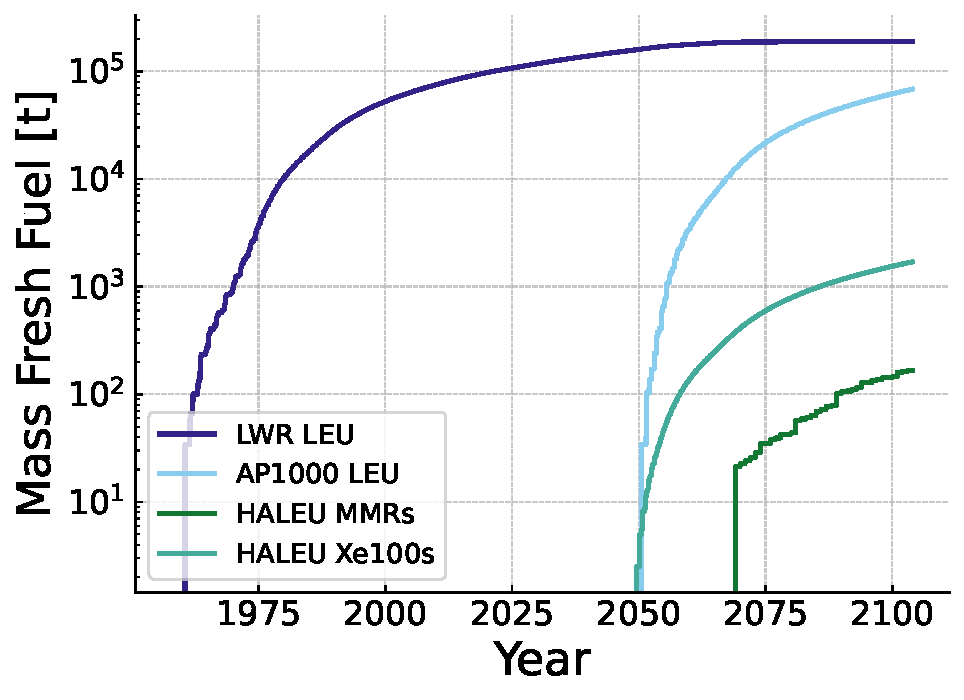
\includegraphics[width=0.495\textwidth]{images/results/used/one_drgng_used_fuel_cumulative_by_fuel.pdf}
   }
    \hfill
    \subfloat[Double. \label{fig:rand_greed_of_d2_used}]{%
      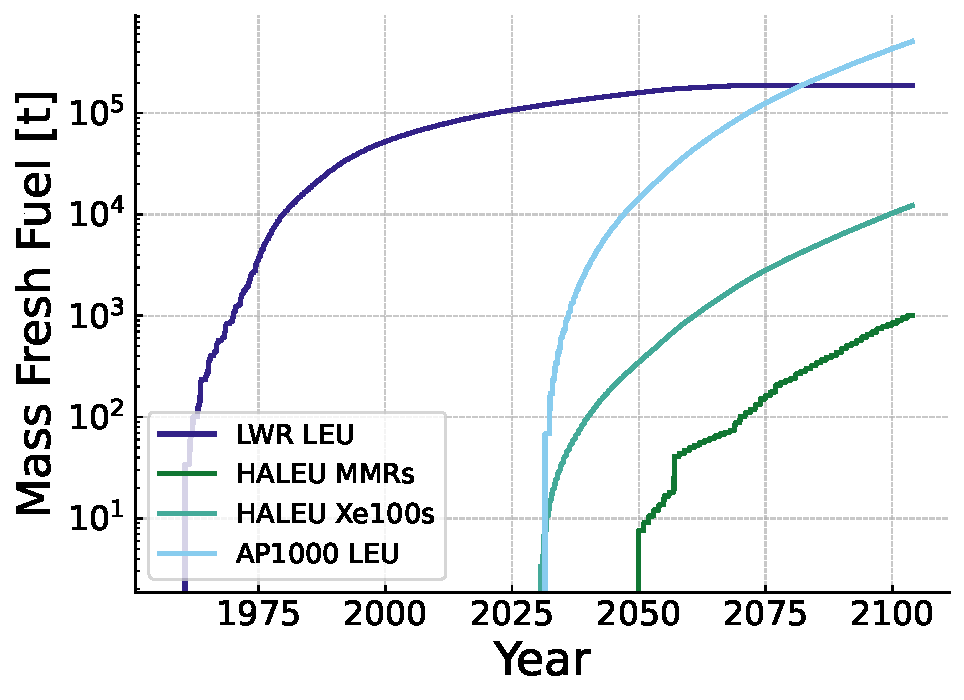
\includegraphics[width=0.495\textwidth]{images/results/used/one_drg2_used_fuel_cumulative_by_fuel.pdf}
   }
    \caption{Initially random, then greedy single used fuel accumulation.}
    \label{fig:rand_greed_of_used}
  \end{figure}


Table \ref{tab:rand_greed_used_avg} shows the average yearly used fuel by design in tonnes for the \textit{no growth} and \textit{double by 2050} scenarios for the multi and single-fuel enrichment deployments. The used fuel demand for the reactors is the same in the single and multi-fuel enrichment deployments for the \textit{no growth} scenarios, which is consistent with the reactor deployment trends in the Section \ref{sec:rand_greed_reactors}. Across scenarios, the demand for used fuel for AP1000 \gls{leu} fuel increases 649\% from the \textit{no growth} to the \textit{double by 2050} scenario in the single-fuel enrichment deployment. The demand for used fuel for \gls{haleu} fuel in the \gls{mmr} and \gls{xe} reactors increases 503\% and 620\% respectively from the \textit{no growth} to the \textit{double by 2050} scenario in the multi-fuel enrichment deployment.

  \begin{table}[H]
    \centering
    \caption{Average initially random, then greedy yearly used fuel by design in tonnes.}
    \label{tab:rand_greed_used_avg}
    \begin{tabular}{l c c c c}
       \toprule
       Scenario & \shortstack{No Growth,\\ Single} & \shortstack{No Growth,\\ Multiple} & \shortstack{Double,\\ Single} & \shortstack{Double,\\ Multiple}  \\
       \midrule
       \gls{mmr} \gls{haleu}   & \textcolor{white}{00}0.185    & \textcolor{white}{00}0.185   & \textcolor{white}{00}1.115    & \textcolor{white}{00}1.063    \\
       \gls{mmr} \gls{leup}    & --       & --      & --       & \textcolor{white}{00}0.052    \\
       \gls{xe} \gls{haleu}    & \textcolor{white}{00}1.882    & \textcolor{white}{00}1.882   & \textcolor{white}{0}13.549   & \textcolor{white}{0}13.419   \\
       \gls{xe} \gls{leup}     & --       & --      & --       & \textcolor{white}{00}0.176    \\
       AP1000 \gls{leu}        & \textcolor{white}{0}75.638   & \textcolor{white}{0}75.638  & 566.239  & 566.239  \\
       \bottomrule
    \end{tabular}
  \end{table}

% talk about repositories
